\section{Estudio de la respuesta de los sensores del robot humanoide TEO y la aplicación de su información al control del equilibrio}

En este capítulo se van a exponer las respuestas de los sistemas sensoriales del robot humanoide TEO a diferentes inclinaciones  para simular perturbaciones pequeñas que cambian la posición del ZMP y mantener el equilibrio del robot haciendo uso de la estrategia de control de los tobillos. Para ello se decidió ajustar un modelo (el modelo de péndulo invertido lineal) de los dos actuales existentes y a partir de él ajustar el otro (el modelo cart-table).

\subsection{Estudio de la respuesta de los sensores F/T}

\subsubsection{Descripción de la metodología experimental}

Para realizar los experimentos ha sido necesario seguir una serie de pasos, ya que si no se seguían los experimentos podrían no dar lecturas correctas y por tanto el experimento sería fallido. Los pasos a seguir son:

NOTA: Los primeros 2 pasos deben realizarse con el robot en suspensión, es decir, sin que toque el suelo con la suela de los pies. A continuación se explicará el motivo.

\begin{enumerate}

%%\item \textbf{Encendido del robot}\\ Encender la fuente de alimentación del robot y el robot junto a sus CPU's, tanto Manipulation como Locomotion.

%%\item \textbf{Iniciar CPU's en el ordenador}\\ Desde el ordenador, deberemos iniciar las CPU's de Manipulation primero y la de Locomotion después, ya que dentro de manipulation se encuentra el YarpServer necesario para la conexión de todos los elementos del robot con el ordenador.

\item \textbf{Puesta del robot en posición inicial (Homeposs)}\\ Una vez se ha encendido el robot y las CPU's se va a proceder a la puesta a cero de la posición del mismo, ya que puede haber modificaciones en su posición de anteriores experimentos o simplemente para asegurarse que los experimentos salen correctamente y siempre empiezan desde la misma posición de inicio. Esto debe realizarse con el robot en suspensión para evitar posibles colisiones de los pies con el suelo.

\item \textbf{Corrección offset sensores F/T}\\ Ya realizada la posición de inicio del robot, desde una terminal se deben iniciar los sensores F/T de los tobillos que se van a encargar de dar la información de las fuerzas y los pares al programa para así poder realizar los experimentos, siempre con el robot en suspensión para eliminar los posibles offset que puedan tener los mismos. Es importante que no esté apoyado en el suelo para que cuando se ejecute esta corrección, no se elimine el valor de la fuerza ejercida por la masa del robot. Una vez que se han iniciado los sensores F/T de los tobillos ya se podría bajar el robot para que éstos puedan tener en cuenta el propio peso del robot y las demás fuerzas y pares. 
%%empiecen a tener el cuenta el peso del propio robot mediante la fuerza de reacción que se genera entre el mismo y el suelo, ya que con él en suspensión los sensores miden pero esas lecturas son de la gravedad.

\item \textbf{Puesta en funcionamiento del programa}\\ Cuando se inicia el programa, existe una primera fase en la que el robot no realiza ningún movimiento. Esto se debe a que se está configurando de tal manera que se elimine el offset que pueda haber al inicio debido a la posición de homeposs del robot, ya que ésta no es perfecta y, debido a la flexibilidad de la estructura y otros errores acumulados, puede no estar totalmente erguido y que las fuerzas en el plano axial no sean cero. 

Una vez que ha pasado esta fase, y estamos seguros de que ese offset se ha eliminado en la medida de lo posible, se envía al robot un $ZMP_{ref}$ y TEO comanda un ángulo, que ha calculado a partir de la conversión del $ZMP_{ref}$, activando los motores de sus tobillos e inclinando el robot dicho ángulo, y calculando el $ZMP_{F/T}$ del modelo de péndulo invertido lineal hasta que este $ZMP_{F/T}$ se estabiliza, para hacer coincidir tanto la parte transitoria como la parte de régimen permanente del $ZMP_{F/T}$ con el del $ZMP_{ref}$.

\end{enumerate}

\begin{figure}[H]
\centering
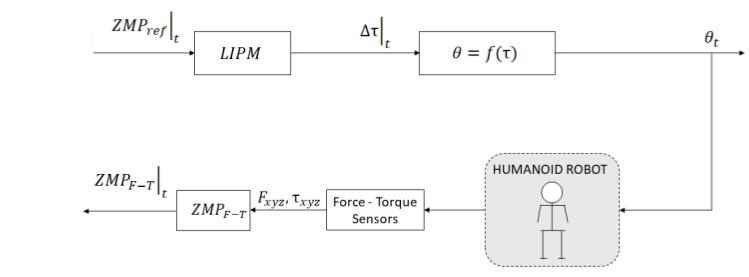
\includegraphics[scale=2.2]{imagenes/apartado_5/5.1/51_esquema1}
\caption{Control de posición básico del ZMP usando el modelo LIPM}
\label{figura51}
\end{figure}

\begin{figure}[H]
\centering
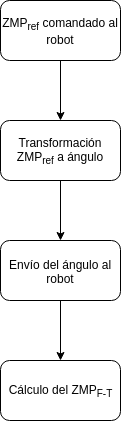
\includegraphics[scale=0.7]{imagenes/apartado_5/5.1/52_diagrama_flujo1}
\caption{Diagrama de flujo del programa}
\label{figura52}
\end{figure}


\subsubsection{Resultados experimentales}

En el presente proyecto se ha llevado a cabo una batería de 30 experimentos.

\begin{figure}[H]
\centering
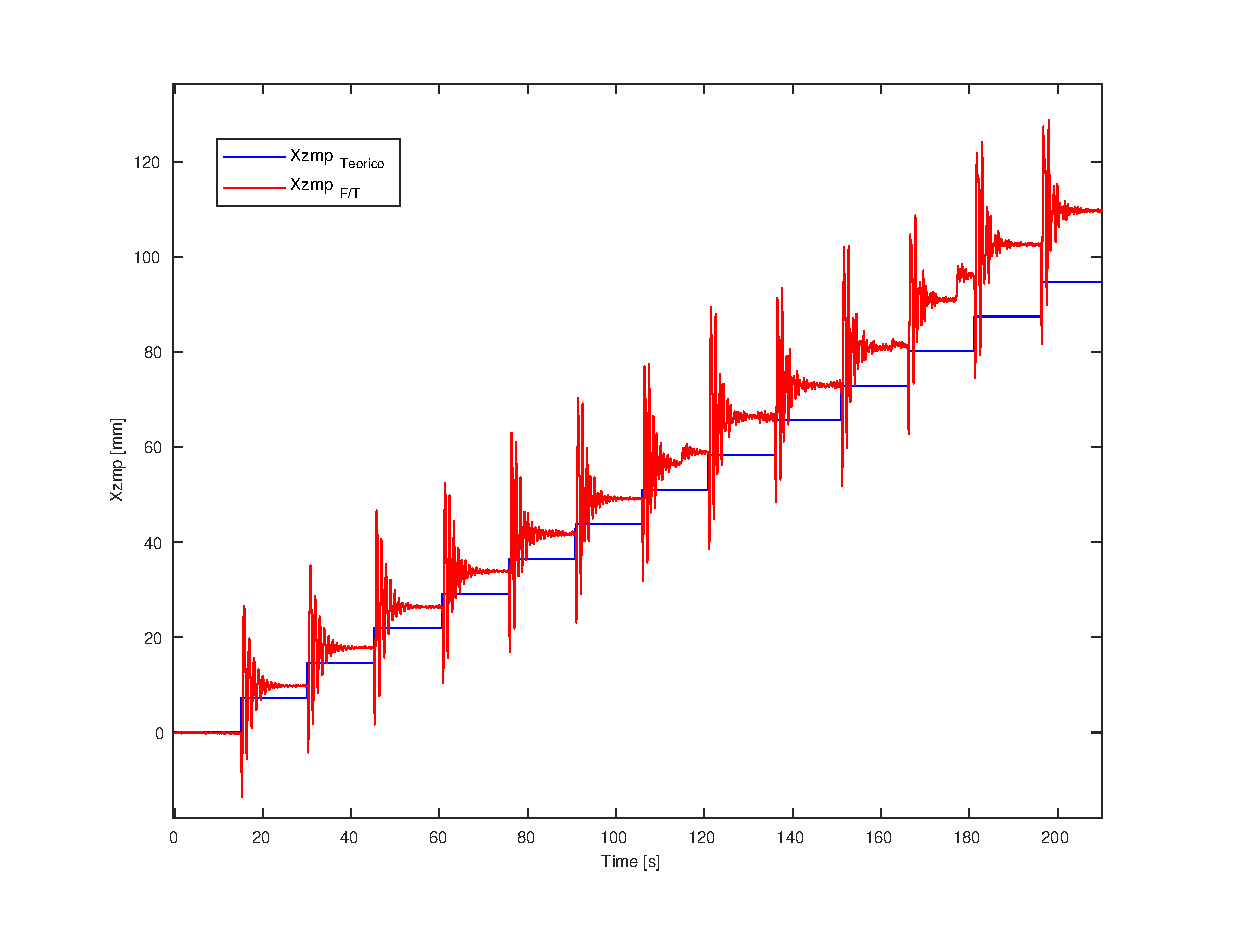
\includegraphics[width=13cm, height=8cm]{imagenes/apartado_5/5.1/53_evolucion_zmp_lipm}
\caption{Evolucion ZMP modelo LIPM}
\label{figura53}
\end{figure}

%%la imagen 53_2 está comentada porque no se si ponerla o no porque en la imagen 53 en el escalón de 9 cm se observa un salto que no me gusta mucho. Puede ser que la prueba no saliera bien por algún motivo que no me acuerdo.

\begin{comment}
\begin{figure}[H]
\centering
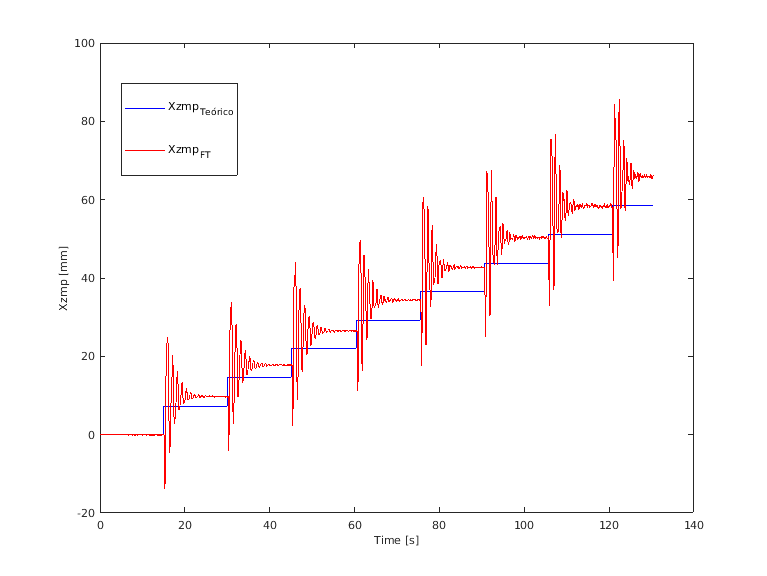
\includegraphics[width=13cm, height=8cm]{imagenes/apartado_5/5.1/53_2_evolucion_zmp_lipm}
\caption{Evolucion ZMP modelo LIPM}
\label{figura53}
\end{figure}
\end{comment}



%aquí introducir la imagen con la evolución de los experimentos

\begin{figure}[H]
\centering
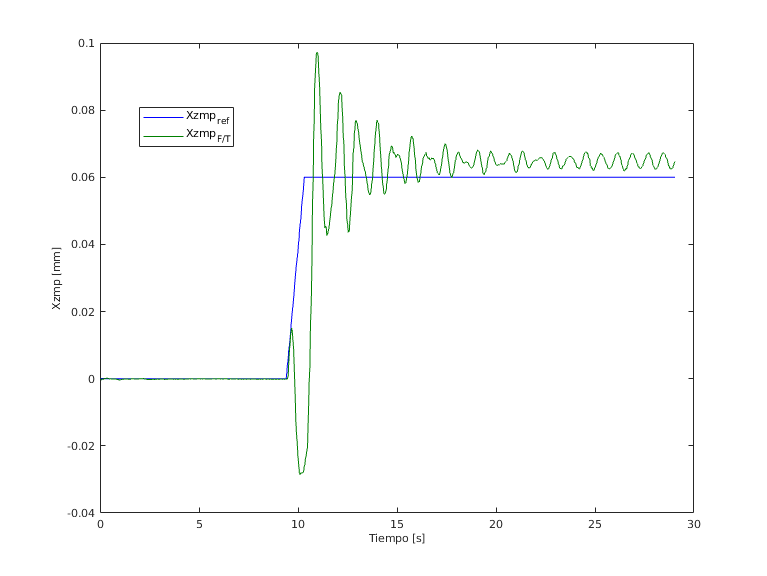
\includegraphics[width=13cm, height=8cm]{imagenes/apartado_5/5.1/54_evolucion_zmpref_5mm}
\caption{Evolución ZMP modelo LIPM para ZMPref = 5mm}
\label{figura54}
\end{figure}

En el gráfico de la figura \ref{figura54} se puede observar que a pesar de realizar un control/corrección sobre el ángulo que se comanda al robot a partir de la conversión del $ZMP_{ref}$, el $ZMP_{F/T}$ nunca llega a estabilizarse y esto es debido a que continuamente se está corrigiendo el ángulo de inclinación.

En los siguientes experimentos se cambiaron varias variables para comprobar si el $ZMP_{F/T}$ se podía estabilizar sin necesidad de un control en el ángulo.

\begin{table}[H]
\begin{center}
\begin{tabular}{|c|c|c|c|}
\hline
Exp. & $k_p$    & $k_d$    & $k_u$ \\ \hline
1    & -0.0025 & 0.00005  & 1    \\ \hline
2    & -0.0025 & 0.00005  & 1.2  \\ \hline
3    & -0.0025 & 0.00005  & 1.4  \\ \hline
4    & -0.0025 & 0.00005  & 2    \\ \hline
5    & -0.005  & 0.0005   & 1    \\ \hline
6    & -0.005  & 0.0005   & 1.65 \\ \hline
7    & -0.01   & 0.0005   & 1    \\ \hline
8    & -0.01   & 0.0005   & 1.65 \\ \hline
9    & -0.05   & 0.005    & 1.65 \\ \hline
10   & -0.015  & -0.00025 & 1.4  \\ \hline
11   & -0.035  & -0.0001  & 1.4  \\ \hline
\end{tabular}
\end{center}
\caption{Batería de experimentos}
\label{tabla51}
\end{table}

\begin{figure}[H]
\centering
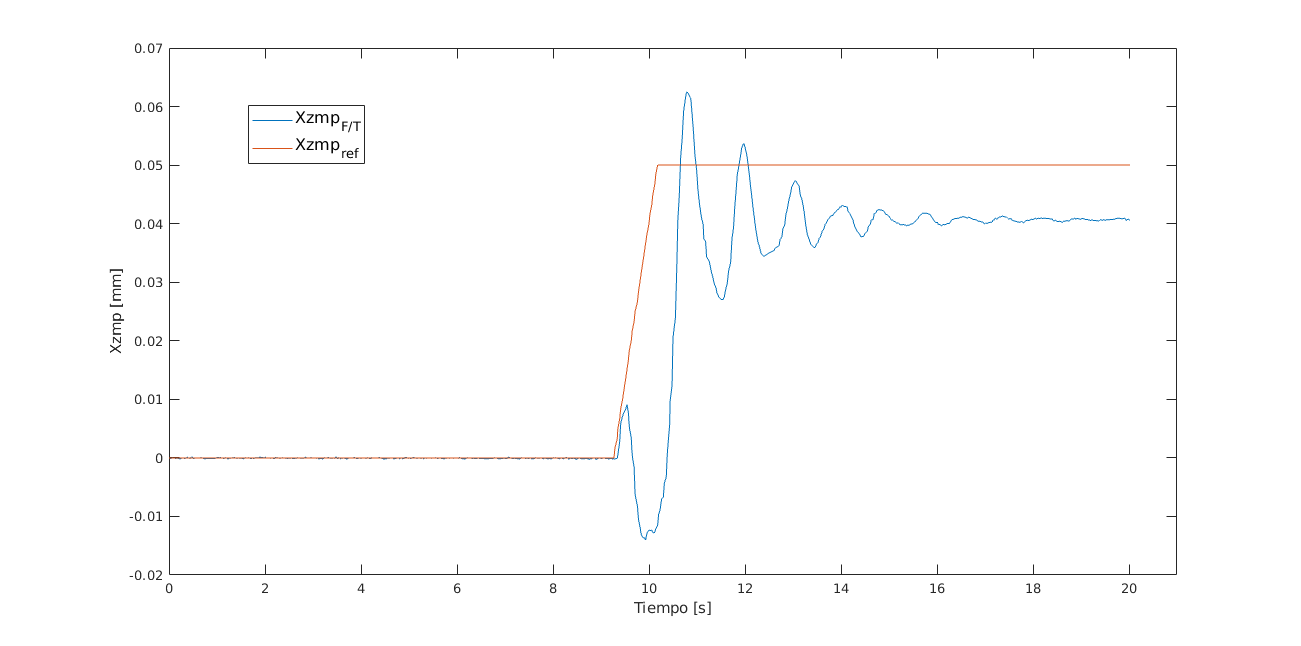
\includegraphics[width=13cm, height=8cm]{imagenes/apartado_5/5.1/55}
\caption{Evolución ZMP modelo LIPM para ZMPref = 5mm}
\label{figura55}
\end{figure}

\begin{figure}[H]
\centering
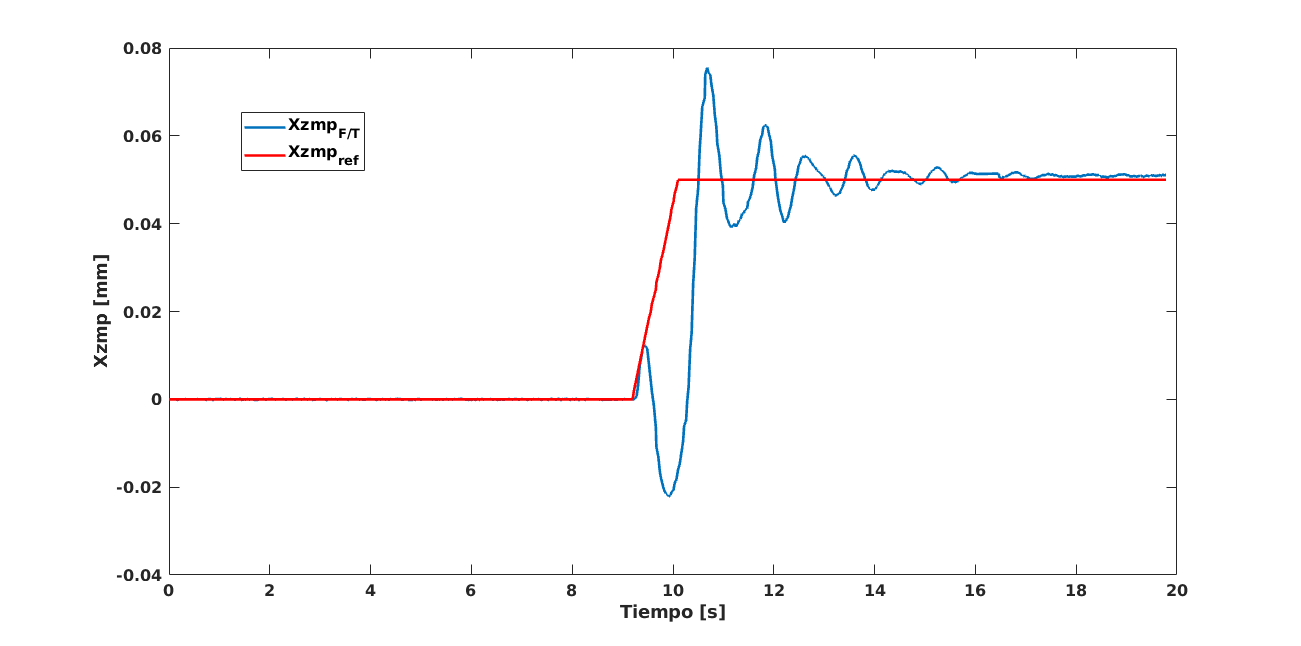
\includegraphics[width=13cm, height=8cm]{imagenes/apartado_5/5.1/56}
\caption{Evolución ZMP modelo LIPM para ZMPref = 5mm}
\label{figura56}
\end{figure}

\begin{figure}[H]
\centering
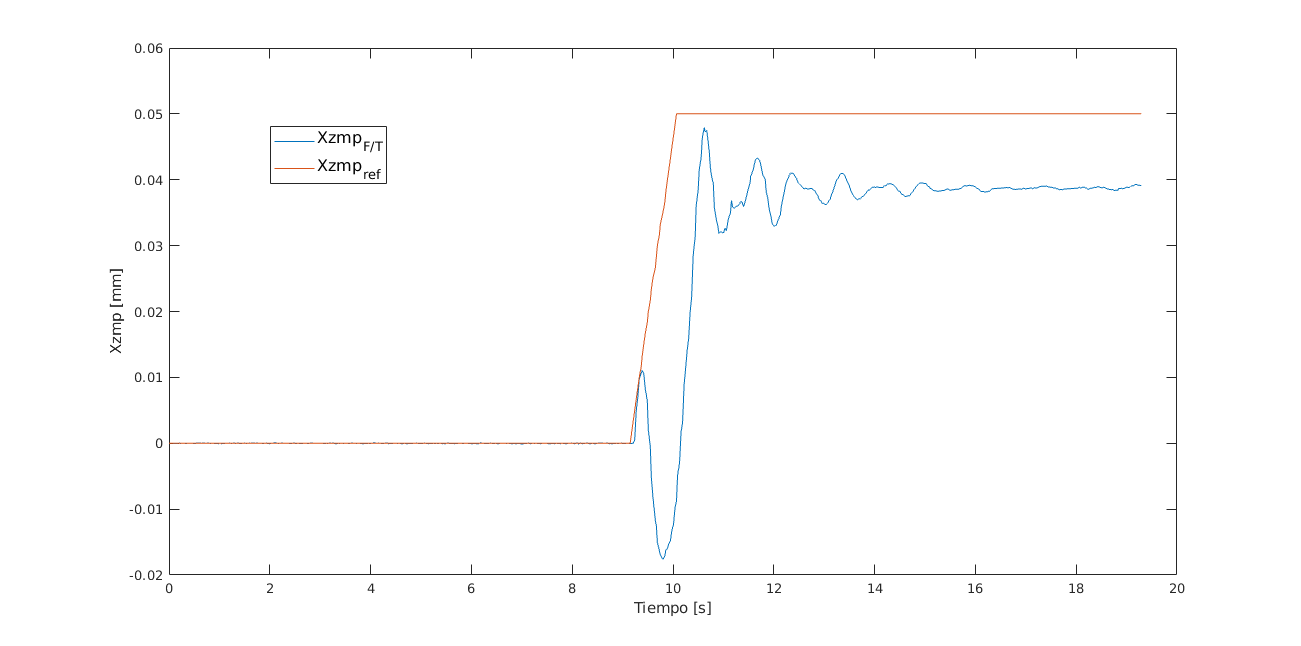
\includegraphics[width=13cm, height=8cm]{imagenes/apartado_5/5.1/57}
\caption{Evolución ZMP modelo LIPM para ZMPref = 5mm}
\label{figura57}
\end{figure}

\begin{figure}[H]
\centering
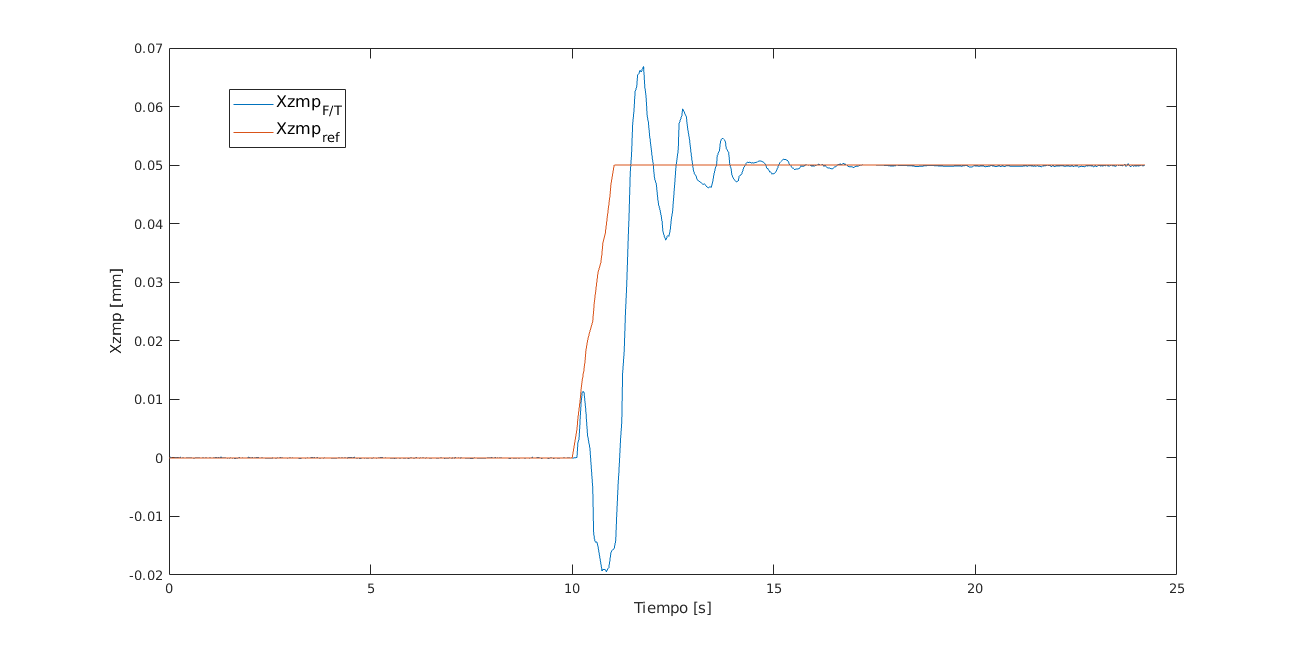
\includegraphics[width=13cm, height=8cm]{imagenes/apartado_5/5.1/58}
\caption{Evolución ZMP modelo LIPM para ZMPref = 5mm}
\label{figura58}
\end{figure}

\begin{figure}[H]
\centering
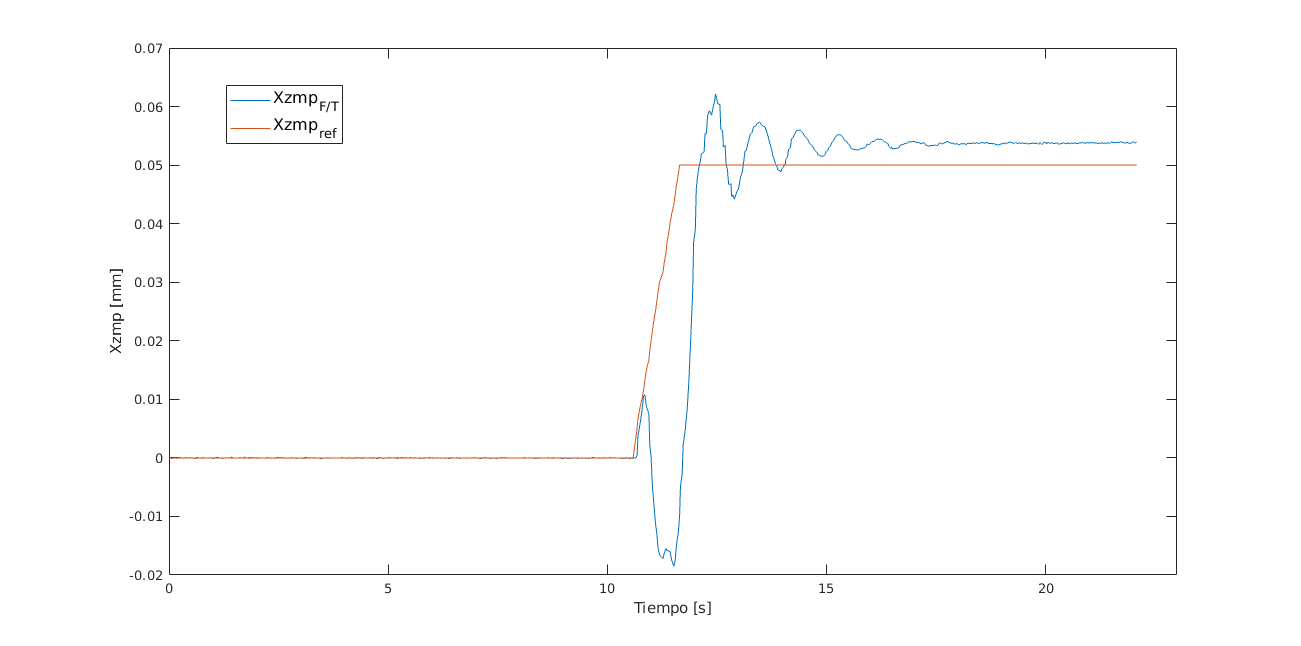
\includegraphics[width=13cm, height=8cm]{imagenes/apartado_5/5.1/59}
\caption{Evolución ZMP modelo LIPM para ZMPref = 5mm}
\label{figura59}
\end{figure}



Las primeras pruebas se desarrollaron en bucle abierto para ver cómo evolucionaba el $ZMP_{FT}$ respecto al $ZMP_{ref}$\footnote{ZMP de referencia al que el robot debería llegar atendiendo a la física y cálculos teóricos del modelo LIPM}, es decir, se comandaba un ZMP de referencia al que tenía que ir el robot y a  partir del esa referencia el robot debía calcular el ángulo de inclinación de los tobillos y una vez que se tenía ese ángulo el robot calculaba el ZMP del modelo LIPM a través de la información que le llegaba de las fuerzas y los pares de los sensores de los tobillos.
 
Como se puede observar el $ZMP_{FT}$ no se corresponde con el $ZMP_{ref}$ conforme se va aumentando el ángulo de inclinación, debido al error que tenía en régimen estacionario. 



Más tarde se decidió realizar las pruebas en bucle cerrado y se puede observar cómo fue mejorando la respuesta del $ZMP_{FT}$ hasta que en la útima gráfica se desarrolló el modelo del actual proyecto, el modelo DLIPM, que se explicará más adelante.

%aquí introducir las gráficas de zmp_ft y zmp_ref frente al ángulo en grados (deg) 


\subsubsection{Modelo Péndulo Invertido Lineal Dinámico (DLIPM)}\label{DLIPM}

Como se ha comentado en el capítulo 4, existen errores provenientes de la información de los sensores F-T de los tobillos del robot debido a los efectos que aparecen en los pares y fuerzas medidos por los sensores cuando éste es sometido a una perturbación de su equilibrio, por lo que se hace necesario separar las inexactitudes de las mediciones y la información relacionada con el comportamiento esperado ante dichas perturbaciones.

Para ello es necesario establecer las variables que intervienen en el proceso (CoM y masa) y definir una estrategia para su control. Para el actual modelo de péndulo invertido lineal aplicado a TEO, la ubicación del CoM y de la masa no son completamente precisas debido a las diferencias entre los diseños CAD y el modelo real del robot, y como ésto no se puede corregir en el robot real, se han utilizado los valores teóricos de dichos parámetros. Para la estrategia de control, teniendo en cuenta el modelo establecido, se puede establecer previamente la ubicación del ZMP para que éste permanezca siempre dentro del polígono de soporte. De esta manera se reducen esfuerzos en el sistema de control, por lo que las ganancias de ajuste serán menores.

A partir de los experimentos desarrollados se ha podido establecer un método para desarrollar el nuevo modelo. Se recogen y procesan los datos obtenidos de los sensores F-T de los experimentos de push-recovery del sistema en bucle abierto. Con esta información, se calcula el $X_{ZMP_{F-T}}$ real y se compara con el $X_{ZMP_{exp}}$ esperado. De aquí se puede observar que hay una diferencia, el error anteriormente comentado, por lo que para corregirlo éste se modela, obteniendo una ecuación para describir dicho error. Una vez obtenido el error modelado, éste se incluye en el modelo original como una fuerza ficticia que corrige la diferencia, obteniéndose el nuevo modelo utilizado a lo largo del actual proyecto. A partir del mismo se puede observar como el comportamiento del ZMP medido y el planificado son similares.

A continuación se van a describir las diferentes fases seguidas para llegar a desarrollar tanto el nuevo modelo como la nueva arquitectura de control y su posterior validación.

\subsubsection{Estudio de la respuesta del sistema}

Para estudiar la respuesta de los sensores F-T ante perturbaciones y aplicar dicha información obtenida al modelo simplificado de TEO, y poder así desarrollar un nuevo modelo personalizado, se ha seguido una serie de pasos divididos en tres fases: fase experimental, fase de análisis de datos y fase de validación de resultados, que se ilustran en la figura \ref{figura510}. 

\begin{figure}[H]
\centering
\includegraphics[scale=0.5]{imagenes/apartado_5/52_diagrama_desarrollo_nuevo_modelo}
\caption{Diagrama del desarrollo experimental del nuevo modelo}
\label{figura510}
\end{figure}

Para poder establecer el nuevo modelo lo primero que hay que hacer es fijar las variables que intervienen en el modelo. La masa del robot TEO es de 62,6 kg y la altura desde el suelo al CoM es 0,893 m (la longitud del péndulo). El siguiente paso que se realizó fue someter al robot a una serie de variaciones en el ángulo de los tobillos para simular perturbaciones pequeñas, con la excepción de que no volvía al ZMP inicial, para así poder modelar mejor la diferencia entre el ZMP esperado y el medido, estudiándose su variación dinámica también a lo largo del proceso. Por último, se validaron los datos para el nuevo modelo con la nueva arquitectura de control.

En la figura \ref{figura511} se presenta al robot apoyado sobre las dos piernas (doble soporte) en un entorno plano orientado hacia el plano en el que se ha desarrollado dicho modelo, el plano sagital (x-z). Esta metodología también se podría aplicar para cualquier otro plano espacial ya que se obtuvieron resultados similares en el plano frontal (y-z). 

\begin{figure}[H]
\centering
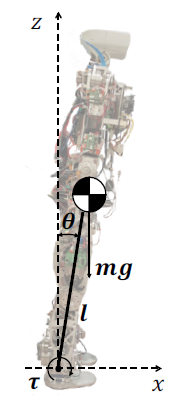
\includegraphics[scale=0.65]{imagenes/apartado_5/53_postura_inicial_experimental_teo}
\caption{Plano de desarrollo de los experimentos del robot TEO}
\label{figura511}
\end{figure}

Las pruebas que se hicieron, con el modelo LIPM, se muestran en la figura  \ref{figura512}, en la que se representa el ZMP medido (señales oscilantes) y el ZMP esperado (señales en forma de escalón). Se sometía al robot a diferentes $ZMP_ref$ a los que debía llegar, transformando dicho ZMP a ángulo para inclinar al robot, y así poder simular diferentes perturbaciones. Como se puede observar, a mayor ZMP el ángulo de inclinación es mayor y el robot es más inestable debido a que éste se encuentra más cerca del borde del polígono de soporte, y los errores tienen mayor influencia, principalmente los que tienen que ver con la flexibilidad de la estructura del robot y sus tolerancias mecánicas. Estos errores se pueden ver en el régimen permanente de la figura. También se observa una oscilación inicial muy grande, algo que se tiene que evitar sobre todo cuando el ZMP se encuentra en el borde del polígono de apoyo. Es por ello que se hace necesario la mejora del control del ZMP, 

%%tanto en régimen permanente, debidos a la flexibilidad de la estructura y sus tolerancias mecánicas, como en régimen transitorio (oscilación inicial de la respuesta del sistema), son mayores.


\begin{figure}[H]
\centering
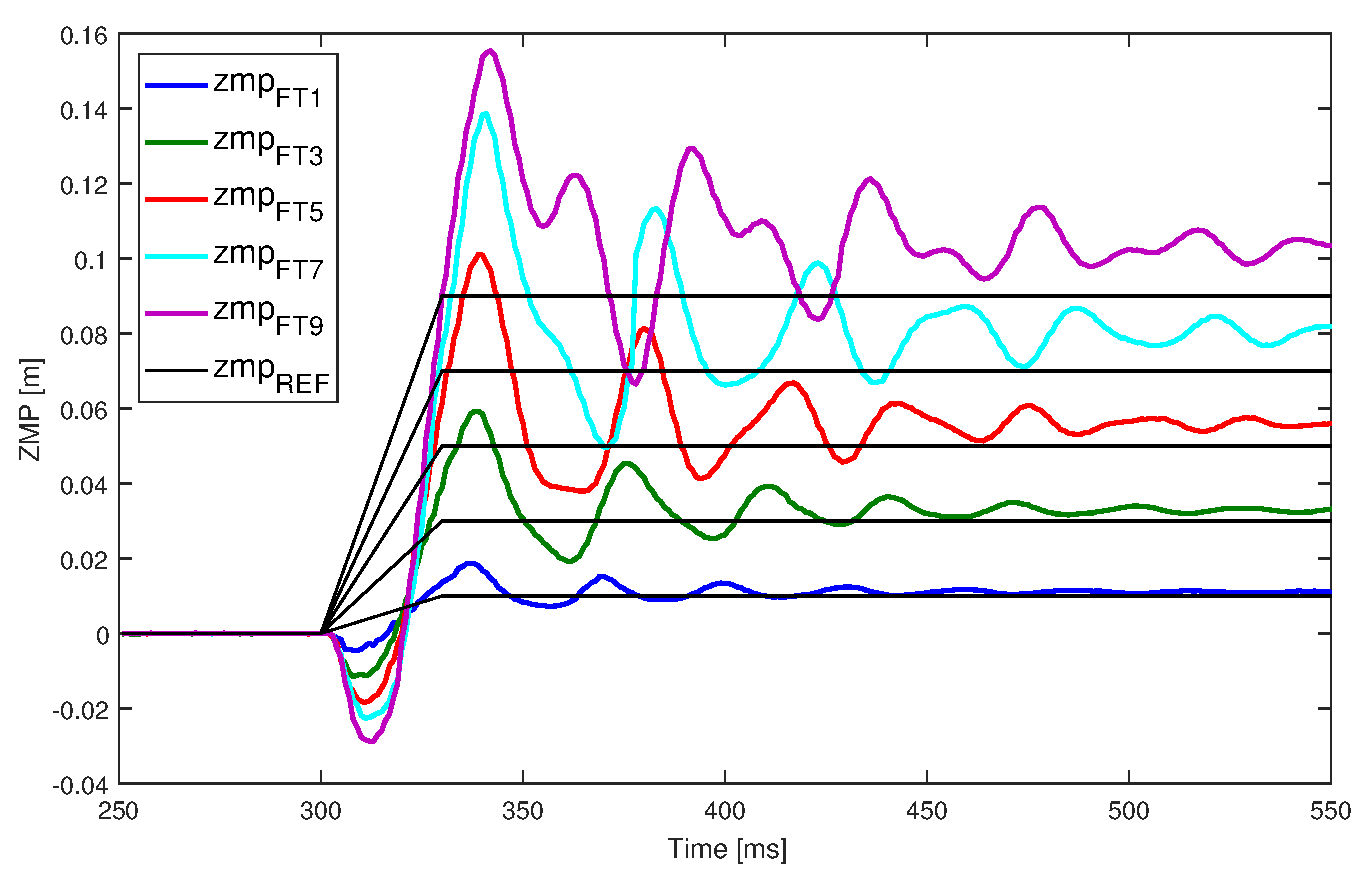
\includegraphics[scale=0.6]{imagenes/apartado_5/5.1/figura3.pdf}
\caption{Evolucion ZMP modelo LIPM}
\label{figura512}
\end{figure}




\begin{figure}[H]
\centering
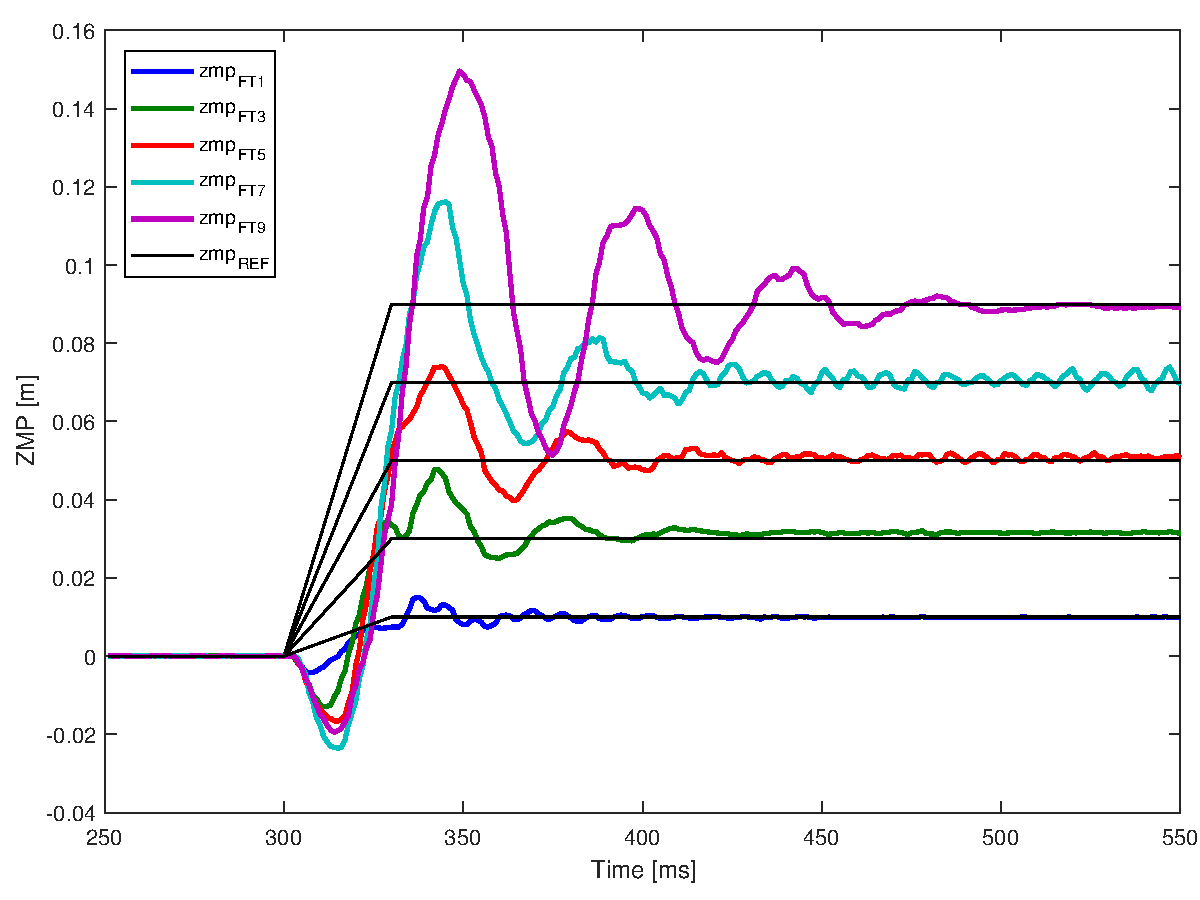
\includegraphics[width=13cm, height=8cm]{imagenes/apartado_5/5.1/figura4.pdf}
\caption{Evolucion ZMP modelo DLIPM}
\label{figura55}
\end{figure}

\subsection{Estudio de la respuesta del sensor inercial IMU}\label{respuestaIMU}



\afterpage{\null\newpage}
\newpage
